\section{Мета роботи}
Мета: Отримати практичні навички та закріпити знання про можливі
подання даних типу рядок та про операції над рядками.
Теми для попередньої роботи:

\noindent
\textbf{Теми для попередньої роботи:}
\begin{itemize}
    \item подання рядків;
    \item операції над рядками;
    \item засоби обробки рядків у мовах програмування;
    \item текстові процесори.
\end{itemize}



\section{Завдання}
Написати програму, в якій передбачити виконання вказаної операції
над рядками за умови подання рядків у пам’яті двома способами.
Порівняти подання рядків вказаними способами за такими показниками:
\begin{itemize}
    \item обсягом використовуваної пам’яті;
    \item часом виконання функції;
\end{itemize}

\noindent
Спосіб подання рядка:
\begin{itemize}
    \item Вектор з керованою довжиною рядка (з дескриптором).
    \item Блочно-зв’язне подання із керованою довжиною.
\end{itemize}

\noindent
\textbf{Функція: }скопіювати з рядка s, починаючи з m-го символу, n символів.



\section{Хід виконання}
Для виконання завдання було обрано мову Rust.
Увесь код також додатково був розміщений в GitHub репозитарії: \href{https://github.com/blackgolyb/algos-labs}{https://github.com/blackgolyb/algos-labs}.


\newpage
\subsection{Vector}
Для цього завдання напишемо власну реалізацю вектора яка буде використовуватися далі
\lstinputlisting[language=Rust, style=colouredRust]{\codeDirectory/src/libs/vector/lib.rs}


\newpage
\subsection{Строка на основі вектора}
Напишемо структуру яка буде реалізовувати строку на основі вектора який состоїть з char.

\noindent
Код програми:
\lstinputlisting[language=Rust, style=colouredRust]{\codeDirectory/src/libs/string/vec.rs}


\newpage
\subsection{Блочно-зв’язне подання строки}
Напишемо Блочно-зв’язну строку яка буде реалізована на основі звязного списка, а елементами буде строка яку ми описали вище.
Також додоамо два способи для розбиття блока:
\begin{enumerate}
    \item Блоку певний розмір,і при перевищені якого буде створюватися новий блок
    \item Блоки розділені певним символом, при попаданні на такий символ буде створено новий блок, а сам символ не буде записаний
\end{enumerate}

\noindent
Код програми:
\lstinputlisting[language=Rust, style=colouredRust]{\codeDirectory/src/libs/string/block.rs}



\newpage
\subsection{Приклад роботи програми}
\noindent
Код програми для перевірки працездатності всіх строк:
\lstinputlisting[language=Rust, style=colouredRust]{\codeDirectory/src/labs/lab6/main.rs}



\begin{figure}[ht!]
    \centering
    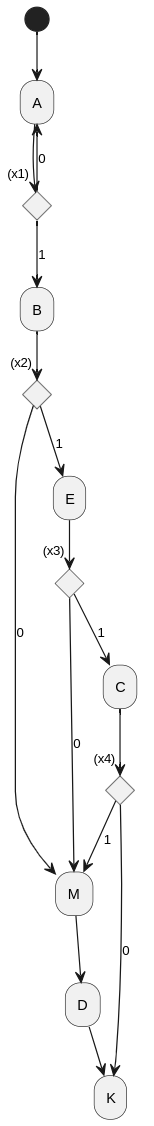
\includegraphics[width=.5\textwidth]{\assetsDirectory/image.png}
    \caption{Приклад роботи}
\end{figure}


\newpage
\section{Висновки}
В ході виконання лабораторної робити було створено 3 варіанти подання строк.
Векторне подання строки є саме ефективне за пам'яттю та за часом виконання операції для подання незмінюваних строк.
В порівнянні векторне подання в 10 разів швидше справляється з тим щоб зробити під строку.
Але блочно-зв’язне подання є також гарним рішенням для дуже великих строк які потребують дуже частих змін,
бо в такому випадку ми можемо вирізати та додавати цілі блоки та не перевиділяти память для змін в рядку.
